% filename: HEP_OP_GEN_TrailerInstallation

\documentclass{article}

\usepackage[utf8]{inputenc}
\usepackage[top=3cm, headheight=2.2cm, headsep=10pt]{geometry}
\usepackage{graphicx}

% To reference the last page
\usepackage{lastpage}

% Like `tabularx` but supports pagebreaks
\usepackage{ltablex}
% Adjust row vertical spacing
\renewcommand{\arraystretch}{1.2}

% Multiline cells
\usepackage{makecell}

% Set date format to ISO 8601
\usepackage{datetime}
\newdateformat{isodate}{\THEYEAR-\twodigit{\THEMONTH}-\twodigit{\THEDAY}}

% Table colouring
\usepackage[table,dvipsnames]{xcolor}
\definecolor{tableHeaderColor}
{rgb}{0.75,0.75,0.75}
\definecolor{tableColumnColor}
{rgb}{0.95, 0.95, 0.95}
\definecolor{notesColor}
{rgb}{0.95, 0.95, 0.95}
\definecolor{highlightColor}
{rgb}{1.00, 0.95, 0.80}

% Icons for checkbox
\usepackage{pifont}

% Command to create a checkbox
\newcommand{\checkbox}{\ding{113}}

% For automatic counters
\usepackage{array}

% Header and footer
\usepackage{fancyhdr}
\pagestyle{fancy}
\fancyhf{} % Clear header and footer
\renewcommand{\headrulewidth}{0pt}
\lhead{\includegraphics[width=2cm]{../../common/assets/HELIOS_LOGO.png}}
\rhead{\includegraphics[width=2cm]{../../common/assets/ARIS_space_to_grow_LOGO-black.pdf}}
\cfoot{\thepage}
\fancyfoot[L]{Project HEPHAESTUS}
\fancyfoot[C]{Page \thepage\ out of \pageref{LastPage}}

% Draft watermark
\newboolean{isDraft}
\setboolean{isDraft}{true} % Set to false to remove the watermark
\ifthenelse{\boolean{isDraft}}{
  \usepackage{background}
  \backgroundsetup{
    scale=25,
    color=gray,
    opacity=0.4,
    angle=45,
    position=current page.center,
    contents={Draft}
  }
}{}

% Highlight colour
\usepackage{soul}
\sethlcolor{magenta}

% Strikethrough
\usepackage[normalem]{ulem}

% Clickable Hyperlinks
\usepackage[colorlinks=true, linkcolor=blue, urlcolor=blue]{hyperref}

% Toggleable procedure items
\usepackage{etoolbox}


% Define a counter for the item numbers
\newcounter{rowCounter}
% Initialize counter
\setcounter{rowCounter}{0}

\newcounter{tableCounter}
\setcounter{tableCounter}{0}

% Command for row in checklist
% First argument is amount
% Second argument is description
\newcommand{\checklistItem}[2]{
  \checkbox & #1 & #2 \\ \hline
}

% Command for row in procedure list
\newcommand{\procedureItem}[2]{
  \stepcounter{rowCounter} % Increment counter
  \arabic{tableCounter}.\arabic{rowCounter}
  &
  \checkbox
  &
  \begin{minipage}[t]{1.2\linewidth}
    #1
    \vspace{1mm} % Just slightly add vspace to prevent clipping into table border
  \end{minipage}
  &
  \begin{minipage}[t]{0.8\linewidth}
    #2
    \vspace{1mm} % Just slightly add vspace to prevent clipping into table border
  \end{minipage}
  \\ \hline
}

% Command for row in note list
\newcommand{\noteItem}[1]{
  \begin{minipage}[t]{\linewidth}
    #1
    \vspace{1mm} % Just slightly add vspace to prevent clipping into table border
  \end{minipage}
  \\ \hline
}


\title{Trailer Installation}
\author{Operating Procedure}
\date{Version: \isodate\today}

\begin{document}

\maketitle

% Set the page style for the title page
\thispagestyle{fancy}

%%%%%% Prefix section
% Change section numbering to A, B, C...
\renewcommand{\thesection}{\Alph{section}}

\section{Operation Description}
 Trailer Installation at Test Site.

\section{Required Tools}
% Table of required tools

\begin{tabularx}{0.9\textwidth}{|>{\columncolor{tableColumnColor}}c|c|X|}
    \hline
    \rowcolor{tableHeaderColor}
    Check & Amount & Description \\ \hline
    \checklistItem{1}{
    \begin{minipage}[t]{\linewidth}
      GTR table clamp 
    \end{minipage}  
    }
    \checklistItem{1}{Pair of gloves}
    \checklistItem{2}{Adjustable wrench (alternatively: SW 21/22)}
  \end{tabularx}

% If no tools required, delete previous lines and uncomment next line
% \textit{none}
  

\section{Required Materials}
% Table of required materials

\begin{tabularx}{0.9\textwidth}{|>{\columncolor{tableColumnColor}}c|c|X|}
    \hline
    \rowcolor{tableHeaderColor}
    Check & Amount & Description \\ \hline
    \checklistItem{1}{Tank Test Setup}
    \checklistItem{1}{Trailer Cable Roll}
    \checklistItem{1}{Fully set-up Mission Control}
    \checklistItem{1}{Funnel}
    \checklistItem{1}{Filling Tube}
    \checklistItem{30L}{Distilled Water}
  \end{tabularx}

% If no materials required, delete previous lines and uncomment next line
% \textit{none}
  

\newpage

%%%%%% Main section
% Change section numbering to 1, 2, 3...
\renewcommand{\thesection}{\arabic{section}}

% Reset section counter to start from 1 again
\setcounter{section}{0}

\section{Trailer Installation}
% Procedure for installation

\stepcounter{tableCounter} % Increment counter
\setcounter{rowCounter}{0} % Reset counter
\begin{tabularx}{\textwidth}{|>{\columncolor{tableColumnColor}}c|>{\columncolor{tableColumnColor}}c|>{\hsize=1.2\hsize}X|>{\hsize=.8\hsize}X|}
  \hline
  \rowcolor{tableHeaderColor}
  ID & Check & Description & Comments \\ \hline

  \procedureItem{Position the trailer such that the wheels are on the edge of the concrete ground. Also check the distance to the Hunter Stübli because of the cable length. Use safety map as orientation. 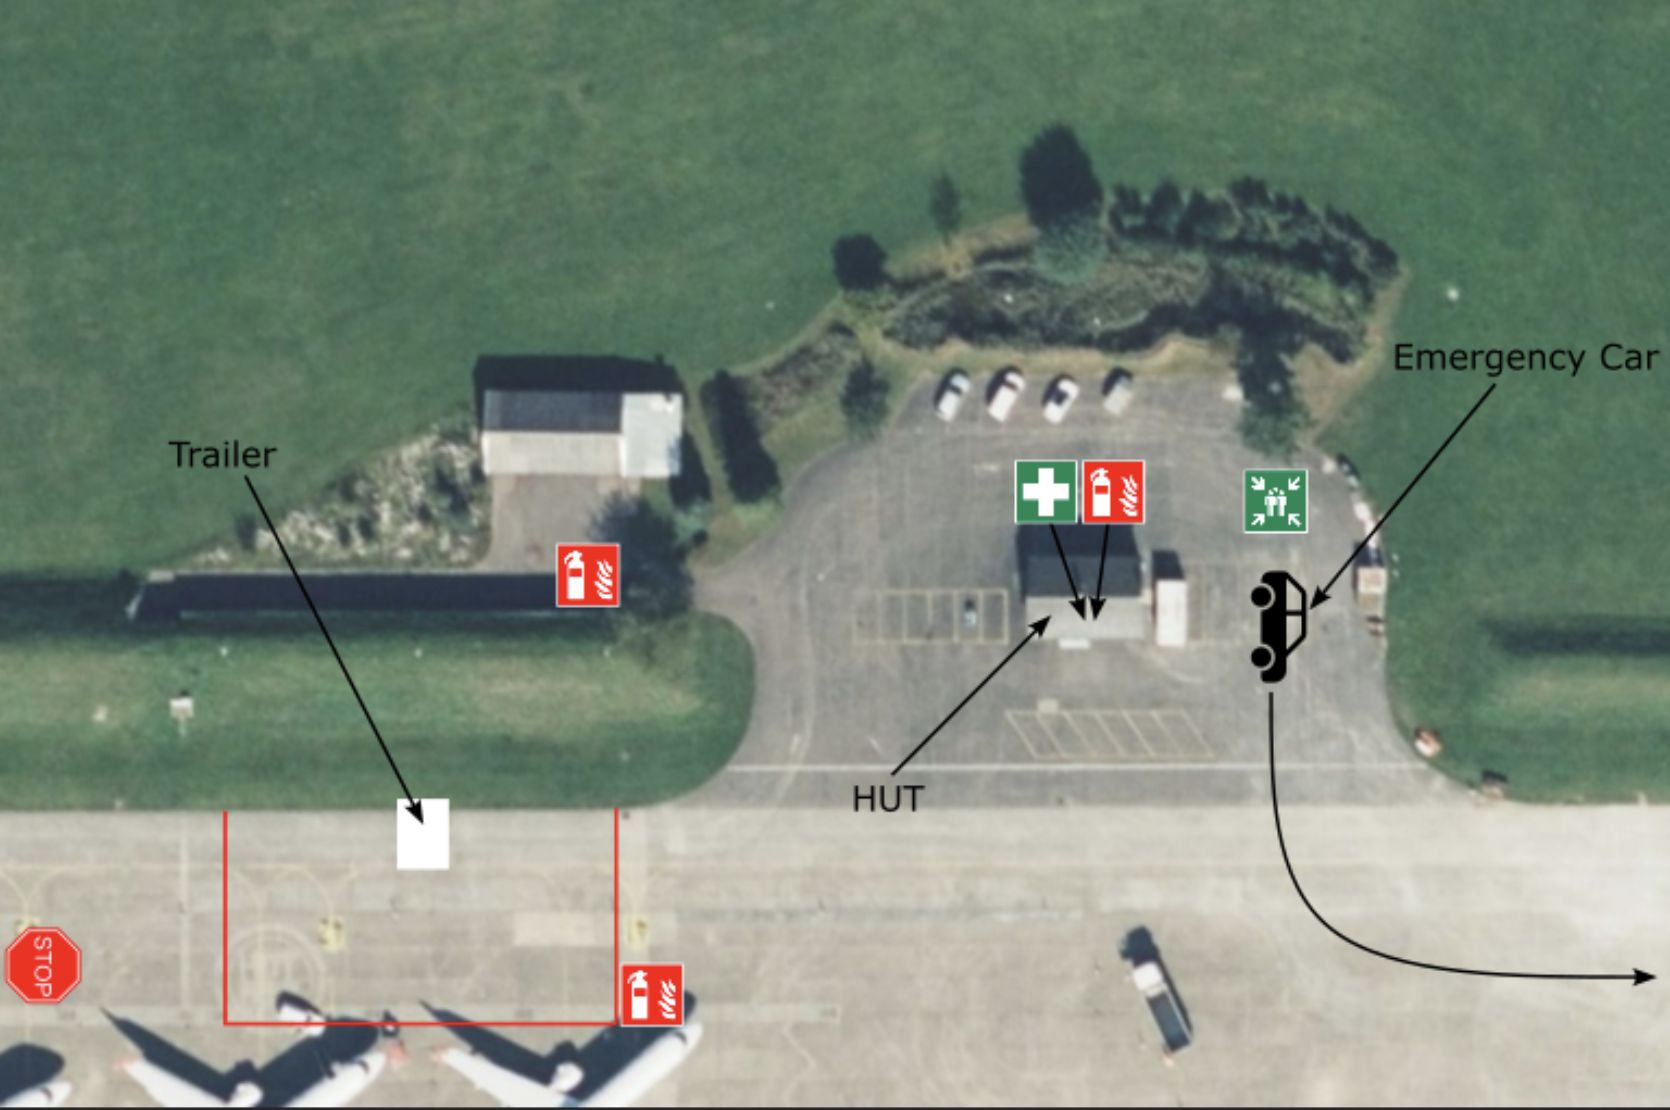
\includegraphics[width=\linewidth]{assets/position_map.png} }{}
  
  \procedureItem{Pull the brake of the trailer}{}
  
  \procedureItem{Put side covers up}{}
  
  \procedureItem{Place the “Riffelblech” on the grass under the front legs.}{}
  
  \procedureItem{Crank down the trailer legs until they carry the weight of the trailer}{}
  
  \procedureItem{Make sure that the shorter side of the Trailer is level (check with level at engine compartment)}{}
  
  \procedureItem{Make sure that the longer side of the Trailer is tilted slightly (mark on level) towards the engine compartment. (Check with level at both sides of the trailer)}{}
  
  \procedureItem{Install fixation cord on the frontside of the trailer by wrapping them once around the metal structures.}{}
  
  \procedureItem{Pull them slightly sidewards to the grass. If Spirafix is not installed: screw Spirafix into the ground where the cords end (hammer may be useful)}{}
  
  \procedureItem{Tighten fixation cord}{}
  
  \procedureItem{Check that trailer fixation is complete}{}
  
  \procedureItem{Inform TC}{}
  
\end{tabularx}


\newpage

%%%%%% Notes
\setcounter{section}{0}
\section*{Notes}
% Notes

\rowcolors{1}{notesColor}{notesColor}
\begin{tabularx}{\textwidth}{X}
  \hline

  \noteItem{}
  \noteItem{}
  \noteItem{}
  \noteItem{}
  \noteItem{}
  \noteItem{}
  \noteItem{}
  \noteItem{}
  \noteItem{}
  \noteItem{}
  \noteItem{}
  \noteItem{}
  \noteItem{}
  \noteItem{}
  \noteItem{}
  \noteItem{}
  \noteItem{}
  \noteItem{}
  \noteItem{}
  \noteItem{}
  \noteItem{}
  \noteItem{.}
  
\end{tabularx}


\end{document}
